% !TeX encoding = UTF-8
% !TeX spellcheck = pt_BR

%Intro começa aqui




\chapter{Uma síntese das transações: da pré-história aos sistemas digitais}
\chaptermark{Uma s\'intese das transa\c{C}\~oes}

\begin{flushright}
	\begin{minipage}{8cm}
		\textit{	\noindent 
			\begin{flushright}
			``Toda troca estimula a atividade produtiva, seja troca por presente, aposta, escambo ou transação com dinheiro.'' - Aaron C. Brown (tradução livre)
			\end{flushright}}
		\vspace{1cm} 
	\end{minipage}
	\footnote{Citação original do inglês: ``All exchange stimulates productive activity, whether exchange by gift, gambling, barter, or money transaction.'' em seu livro \cite{WALLSTREET}}.
\end{flushright}


Neste capítulo será apresentado um breve resumo histórico de como eram as realizadas as transações mostrando as bases do dinheiro que conhecemos hoje. 

\section{Prólogo}

Ah, o dinheiro. Se o digníssimo leitor começasse a imaginar especificamente sobre este termo, muito provavelmente seus primeiros pensamentos seriam sobre todos os benefícios que este pode oferecer, digamos viagens para as mais belas paisagens disponíveis mundo afora, seja uma noite amena em um jantar requintado, um feriado em uma megalópole, além de muitas outras localidades. Alguns de nossos leitores também poderiam se encontrar imaginando notas de real, notas de euro, notas de dólar e moedas, outros ainda cartões de crédito e débito, vale refeição e alimentação. Arrisco ainda dizer que os ainda mais jovens pensariam na forma do dinheiro que se quer tocamos, que pode ser transferido digitalmente, com uso de ferramentas regulamentadas, como o PIX, por exemplo.  O conceito de moeda \footnote{Uma definição de dinheiro, segundo \cite{KRUNGMAN} "O dinheiro, argumentaram os economistas clássicos, serve a três funções: é um meio de troca, uma unidade de conta e uma reserva de valor".}\footnote{Uma definição bastante formal sobre dinheiro usada na escola austríaca de economia fica a cargo de \cite{MISESA}:"Assim, haveria uma tendência inevitável para os menos comercializáveis ​​da série de bens usados ​​como meio de troca devem ser rejeitados um por um até que, finalmente, apenas uma única mercadoria permaneceu, que foi universalmente empregada como um meio de intercâmbio; em uma palavra, dinheiro".}\footnote{ Se tormarmos uma abordagem mais filosófica, veremos que nem tudo são um mar de rosas. Segundo o apóstolo Paulo no primeiro livro de Timóteo afirma que o amor ao dinheiro é a raiz de toda a espécie de males; causador da cobiça de alguns que se desviaram da fé, e com muitas dores se traspassaram \cite{BIBLE1}.} que conhecemos hoje não é o mesmo de tempos remotos da passagem humana pelo planeta terra. Com efeito, se a pessoa mais rica do nosso país viajasse no tempo levando consigo sacolas com grande quantidade de dinheiro e se encontrasse com os humanos primitivos antes da era paleolítica, muitos deles veriam naquele montante somente alguma matéria prima para ser queimada e com isso obter uma fonte de calor para se proteger do frio. Tal diferença nas percepções de um mesmo objeto mostra o progresso da evolução humana, no qual neste tempo, este teve inúmeras alterações em sua estrutura no objetivo de satisfazer as necessidades sociais da população. Vejamos a seguir alguns momentos que foram fundamentais para esta evolução. 

\section{O princípio}

\subsection{Escambo}

Em uma época onde não havia um objeto que por exemplo, se pudesse trocar uma saca de arroz por este que mais tarde seria trocado por outro produto, um galinha, por exemplo. Chamamos este objeto inexistente da época de moeda fiduciária (do inglês \textit{Fiat Money}\footnote{\label{fiat} Segundo \cite{GOLDBERG}, o dinheiro fiduciário é uma moeda (um meio de troca ou transação) estabelecida como dinheiro, geralmente por regulamentação governamental. A moeda, de forma fiduciária, não tem valor intrínseco e não tem valor de uso. Tem valor apenas porque um governo mantém o seu valor ou porque as partes envolvidas na troca concordam com o seu valor.}) Nesta época as transações se baseavam em trocar bens por bens, bens por serviços ou serviços por serviços. Usando o exemplo que vimos anteriormente, há então duas possibilidades, se um criador de animais tivesse o desejo de se obter uma saca de arroz, este deveria então encontrar alguém que tivesse em suas propriedades uma produção de arroz e ao mesmo tempo ter interesse em adquirir animais, ou então deveria produzir seu próprio arroz. Como se pode perceber, nos deparamos com um primeiro problema, que podemos chamar de conflito de interesses. Qual a possibilidade de se encontrar alguém que tenha interesse em trocar certos commodities comigo, na quantidade que estou oferencendo? Tal limitação traria dificuldade no desenvolvimento econômico e tecnológico desta população. 

\begin{figure}[H]
	\centering
	\caption{Escambo: Um acordo entre duas partes}
	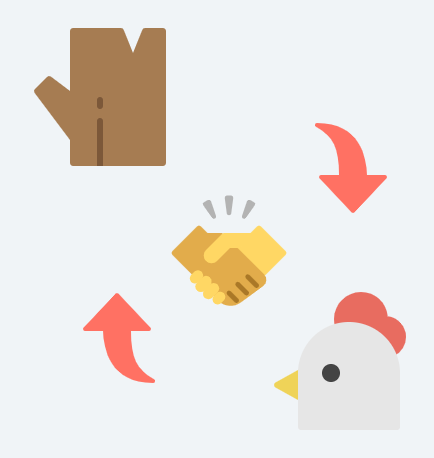
\includegraphics[width=0.5\linewidth]{barter_1.png}
	\text{Fonte: Desenvolvido pelo autor com assets disponíveis em \cite{WHIM}}\\
\end{figure}

\subsection{Conchas (e outros objetos)}
Este foi um dos benefícios da ideia da objetificação monetária, que além de servir como um fomentador para a economia, permitiu a realização  dos mais diversos tipos de transações, além de uma especialização da mão de obra. De fato, um lenhador poderia adquirir vestimentas, ferramentas e alimentos sem necessariamente ter que procurar alfaiates, ferreiros e fazendeiros que tenham interesse em madeira para isso pois a moeda passou a ser mais aceita pela população, permitindo escambos com um maior número de itens. Com isso, o lenhador não precisaria desenvolver suas próprias vestimentas e ferramentas e se especializar com técnicas de melhor extração de madeira e plantio de mais árvores, por exemplo. \footnote{Na figura \ref{intro_money}, a moeda de troca foi representada por uma moeda dourada, mas note que ainda não haviam moedas no tipo.  Veremos mais sobre os metais na seção \ref{metals} abaixo}

\begin{citacao}
	Embora possam parecer uma escolha bastante aleatória, as conchas tinham uma série de vantagens: eram semelhantes em tamanho, pequenas e duráveis. Enquanto os moluscos que produzem as conchas são encontrados nas águas costeiras dos oceanos Índico e Pacífico, a expansão do comércio fez com que até alguns países europeus aceitassem conchas como moeda. Conchas na forma de wampum (contas tubulares de conchas) foram usadas como dinheiro pelos nativos americanos. \cite{BRIT}
\end{citacao}

\begin{figure}[H]
	\centering
	\caption{Introdução ao dinheiro}\label{intro_money}
	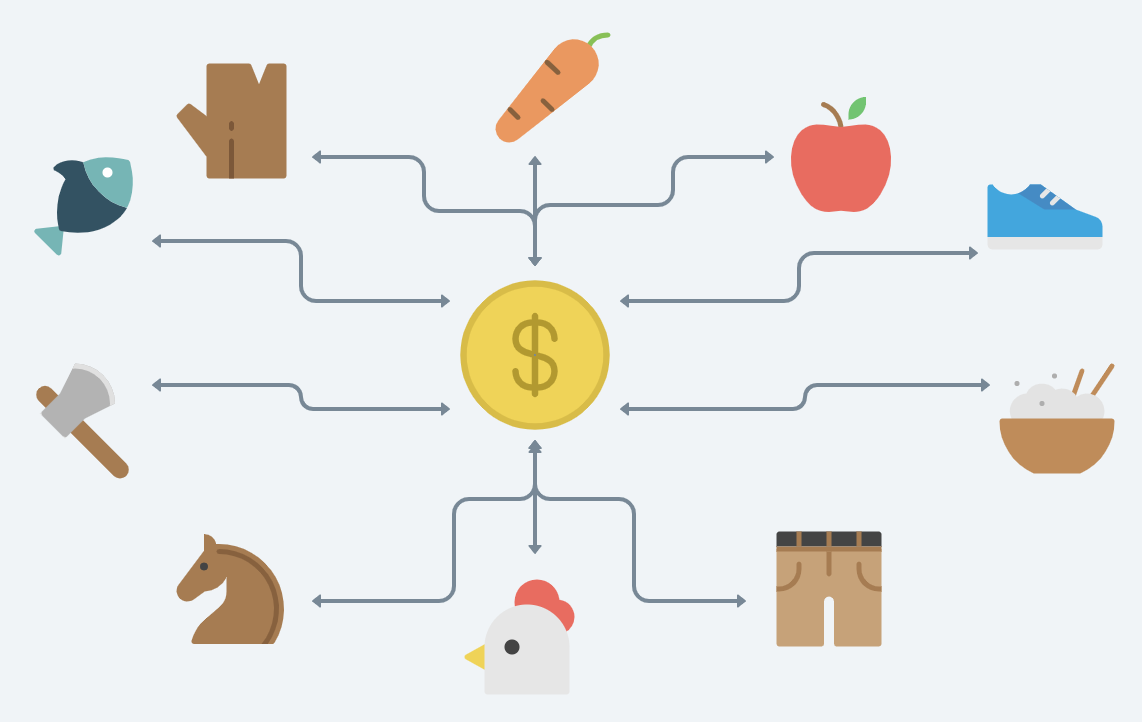
\includegraphics[width=0.8\linewidth]{barter_2.png}
	\text{Fonte: Desenvolvido pelo autor com assets disponíveis em \cite{WHIM}}\\
\end{figure}



Perceba que não havia inicialmente um único tipo de moeda, uma lista longa de objetos serviu como moeda ao avançar dos tempos, sendo eles grãos de arroz, dentes de animais, animais e até escravos. Estes além de servir como forma de pagamento também tinham dois papeis importantíssimos: permitir a movimentação de recursos entre regiões mais afastadas geometricamente e também fixar os preços de todos os bens para uma única unidade. Ao passar do tempo, mais especificamente próximo do século VI A.C. as moedas metálicas foram tomando o lugar destes objetos devido a sua durabilidade, tamanho facilidade de divisão em partes menores e facilidade de transporte. 


\section{A jornada dos metais}\label{metals}

Não poderíamos iniciar esta seção sem citar a numismática\footnote{Segundo o dicionário Dicio, numismática é a ciência que se dedica ao estudo de medalhas e moedas; numária ou numulária. Não só a ciência por trás deste estudo mas também pode ser relacionado como sinônimo ao colecionismo de tais moedas e medalhas. \cite{DICIONUM}}, que é exatamente a área de estudo que trata do assunto aqui abordado. Continuando,  artefatos metálicos, em sua majoritária parte obtiveram alta popularidade como meio de troca devido sua portabilidade, durabilidade e divisibilidade\footnote{ Para facilitar a compreensão do leitor, tome nota do seguinte exemplo: uma moeda de hoje como 1 (um) BRL (um real brasileiro). Perceba que este pode ser dividido em 100 partes de centavo, cada uma valendo R\$ 0,01. Imagine a dificuldade e impraticabilidade de se dividir um animal vivo, como um boi, em incrementos pequenos o suficiente para realizar um escambo, ou como moeda de troca por um ramo de cenouras, por exemplo. Casos como estes são outra razão da popularidade dos metais em detrimento de peças vivas como animais, possibilitando assim espaço para a evolução da sociedade.}, trazendo consigo as origens da cunhagem\footnote{Segundo o dicionário Priberam, a cunhagem refere-se ao ato ou efeito de cunhar. Já cunhar refere-se ao ato de imprimir cunho num metal, originando moeda (ex.: cunhar euros; cunhar moeda), ou simplemente transformar em moeda (ex.: cunhar prata)\cite{PRIBERAM1}}. Dependendo da região, a escolha do metal era determinada pela disponibilidade de acordo com esta região.
No Egito antigo, apesar de não adotarem o uso de moedas de anéis de ouro no comércio exterior até o final do século 4 D.C., utilizavam barras de ouro desde o 4o milênio A.C., que mais tarde acabaram se desenvolvendo. Próximo ao Mar Egeu, ​​lingotes de cobre conhecidos como talentos, eram originalmente uma unidade de peso de aproximadamente 55 a 70 libras (algo entre 25 kg e 31 kg) foram usados ​​como moeda vários séculos antes da cunhagem. Na grécia, a descoberta de uma barra de ferro com um punhado\footnote{Também conhecido como dracma} de espetos de ferro fracionários\footnote{Cujo nome é dado por obelois} serviu como moeda próximo de 1100 A.C. . Ainda há outros exemplos de "moedas pesadas" também conhecidos como talentos\footnote{Segundo \cite{HUMPHREY}, o peso aproximado de um talento poderia variar de acordo com a região. Por exemplo, um talento grego, pesava 20,04kg (57 lb); um talento egípcio 27 kg (60 lb) e um talento romano pesava 32,3 kg (71 lb)}. Ao prosseguir da história, nota-se o desejo de subdividir uma unidade pesada em frações menores para uso normal. \\

\subsection{Cunhagem}
Já segundo relatos históricos, a China foi o primeiro país a utilizar em suas transações objetos nos quais eu e você, caro leitor, reconheceria como um moeda. . Ainda assim, objetos como cochas confeccionadas por mãos humanas com materiais como o bronze, já existiam. Aqui estamos falando de 770 A.C. . Segundo citação de \cite{CHINA} no livro "Moedas chinesas: Dinheiro na história e na sociedade" (Tradução nossa):

\begin{citacao}
 À medida que o comércio se desenvolveu ainda mais e as fronteiras geográficas do comércio foram alargadas, a demanda por conchas naturais aumentou, e logo as conchas por si só não foram suficientes para atender à demanda. Em seguida, apareceram conchas de imitação criadas a partir de materiais feitos pelo homem. Um exemplo é a concha de bronze. Como as conchas de bronze eram facilmente unificadas em tamanho, peso e valor, elas foram imediatamente reconhecidas como superiores às conchas naturais. O aparecimento de conchas de bronze marcou o início da cunhagem de metal, que foi um grande passo à frente no desenvolvimento da economia jin. Devido ao rápido desenvolvimento econômico na primavera e outono e no Período dos Reinos Combatentes (770-221 a.C.), apareceram vários tipos de moedas. A forma de tais moedas imita formas de ferramentas agrícolas ou itens encontrados na vida diária. (Tradução nossa)
	\end{citacao}

\subsection{A primeira moeda oficial}
Já a primeira região do mundo a usar procedimentos e instalações "industrializadas" para fabricar moedas que poderiam ser usadas como moeda de troca foi na região chamada Lídia, o que hoje seria considerada atualmente como Turquia ocidental, na europa. E ainda na Lídia, sob o reinado do rei Alyattes  por volta de 610 A.C. surgiu o  "Leão Lidiano"\footnote{Aqui estou fazendo uma tradução livre. Diversos textos em língua inglesa afirmam o nome "Lydian Lion" para a primeira moeda do mundo enquanto há poucas referências em português citando um nome para a moeda, referindo-a apenas como um estáter.},a primeira moeda oficial, justante cunhada com a efígie de um leão, símbolo da família real da Lídia, segundo os numismáticos. As moedas eram feitas de electro, uma liga ou mistura de origem natural de prata e ouro, e as vezes com vestígios de platina, cobre e outros metais. \footnote{Você pode ler sobre este assunto em \cite{MONTEREY}}

\begin{figure}[H]\label{lydian1}
	\centering
	\caption{O "Leão Lidiano", a primeira moeda}
	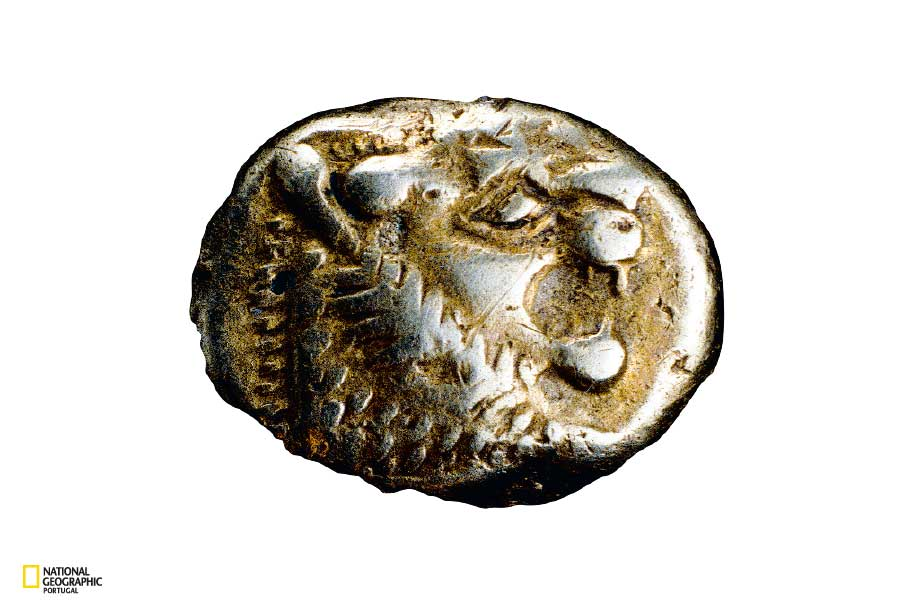
\includegraphics[width=0.7\linewidth]{lydian_lion.jpg} 
	\text{Fonte: \cite{LLION}}\\
\end{figure}
\begin{figure}[H]\label{lydian2}
	\centering 
	\caption{Mapa da Lídia de 1903}
	\includegraphics[width=0.7\linewidth]{lydia_map.jpg}\\
	\text{Fonte: \cite{LMAP}} 
\end{figure} 

\section{A transição para o papel moeda}

Somente ao findar da dinastia Tang (618-907 D.C.) até a dinastia Song (960-1279 D.C.) ao iniciar do século VII na China pré-moderna é que o papel moeda surgiu como um meio de reduzir a necessidade de transportar as pesadas e incômodas moedas metálicas vistas até aqui para realizar transações. Se compararmos com os banco modernos, muito semelhantemente  depósito eram feitos em entidades de confiança, e somente aí recebiam uma nota indicando quanto dinheiro haviam depositado. A nota poderia então ser resgatada em moedas de ouro e prata em uma data posterior. Segundo citação de \cite{BRIT}: (tradução nossa):

\begin{citacao}
	Era feito da casca das amoreiras (então, em certo sentido, o dinheiro realmente crescia nas árvores). No final do século 18 e no início do século 19, o papel-moeda se espalhou para outras partes do mundo. O grosso dessa moeda, entretanto, não era dinheiro no sentido tradicional. Em vez disso, serviu como notas promissoras - promessas de pagar quantias específicas de ouro ou prata - que foram fundamentais para o desenvolvimento dos bancos.
	\end{citacao}

Note que estes também poderiam ser trocados por bens e serviços e que eram emitidos por bancos e instituições privadas, não pelo governo, que agora é responsável pela emissão de moeda na maioria dos países segundo \cite{BRIT2}. O papel moeda ainda perdurou por 500 anos até que a prática começasse a se popularizar na Europa no século 17. Ainda, o primeiro papel-moeda emitido por governos europeus foi, na verdade, emitido por governos coloniais na América do Norte. Relata-se que os colonos muitas vezes ficavam sem dinheiro à medida que as operações se expandiam pois os carregamentos entre a Europa e as colônias da América do Norte demoravam demasiadamente.\footnote{Voce pode ler mais sobre isto em \cite{TEXAS}} Com isso, em vez de voltar ao sistema de troca, os governos coloniais emitiam cartas assinadas\footnote{Em inglês, um tipo deste documento é conhecido como IOU, documento que faz o reconhecimento da existência de uma certa dívida. Seu nome é uma fonética para "I owe you" (eu lhe devo, em portugês). Leia mais sobre isto em \cite{KENTON}} com valores intrínsecos que passavam a ser negociados como uma moeda.

\begin{figure}[H]\label{card}
		\caption{Cartas assinadas}%
		\subfloat[\centering Carta de baralho assinada por entidade governamental para uso como moeda,1729]{{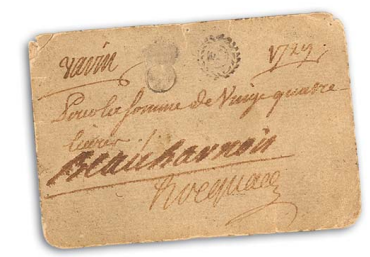
\includegraphics[width=0.5\linewidth]{card_money.png} }}%
		\quad
		\subfloat[\centering Regime francês, Reprodução de (a), 1714]{{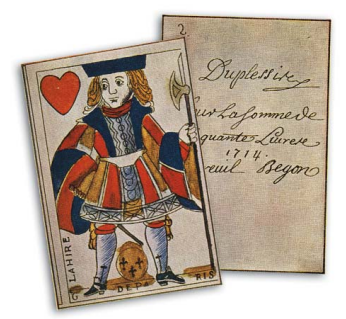
\includegraphics[width=0.5\linewidth]{card_money2.png} }}%
		\begin{center}
			\text{Fonte: \cite{CANADA}}\\
		\end{center}
\end{figure}

\section{Guerras cambiais}
Com a definitiva mudança para o papel moeda na Europa, os bancos e as classes dominantes começaram então a adquirir moedas de outras nações e criaram o primeiro mercado de câmbio, impulsionados pelo aumento das quantidades de transações internacionais possíveis. A capacidade dos países de negociar eram baseadas na estabilidade de seu governo ou monarquia, afetando assim o valor da moeda de sua nação. Isto acabou gerando competições entre os países, levando diversas vezes a guerras cambiais \footnote{Segundo o jornal BBC \cite{BBC1}, o termo Guerra cambial é usado por diversos governos e economistas para descrever uma suposta disputa entre os países envolvendo suas moedas. O argumento é de que alguns países estariam impondo a desvalorização de suas moedas para beneficiar seus ganhos com exportação. Também pode referir-se como "Guerra monetária" e Guerra das moedas}, em que os países concorrentes encontravam métodos de alterar o valor da moeda do país concorrente elevando-a, encarecendo os bens do inimigo, reduzindo assim seu poder de compra\footnote{Considere aqui também a capacidade de pagar para uma guerra, conforme visto no exemplo logo a seguir}. Tome por exemplo a seguinte citação em \cite{KEYNES}:

\begin{citacao}
	Um dos primeiros exemplos da aplicação do argumento do desemprego como uma razão para a proibição das importações foi encontrado em Florença no ano de 1426. $(\cdots)$ Numerosos ataques foram dirigidos contra todas as pessoas que deveriam ter contribuído para uma exportação (excedente de exportação) de metais preciosos, ou para seu desaparecimento por causa de atividades correspondentes no país. (Tradução nossa)
\end{citacao}

O trecho é um exemplo do mercantilismo\footnote{Segundo \cite{TODAMAT} O Mercantilismo foi o conjunto de ideias e práticas econômicas com objetivo de que aa fonte de riqueza de uma nação se baseava no comércio com o mercado exterior e no acúmulo de metais preciosos.}, que ocorria quando as nações desejavam competir economicamente, envolvendo práticas para aumentar as exportações enquanto limitavam-se as importações. Com o desejo de aumentar a oferta de moeda doméstica e a riqueza das autoridades governantes, acontecendo especialmente por causa da necessidade de financiar guerras ou pagar dívidas, ocorria então a desvalorização da moeda.

Note que esta competitividade cambial ocorre até hoje, sendo um dos frutos de estudo de macroeconomia e preocupa investidores que têm interesse em fundos cambiais.

\begin{figure}[H]\label{notes}
	\centering
	\caption{Exemplos de moedas fiduciárias atuais}
	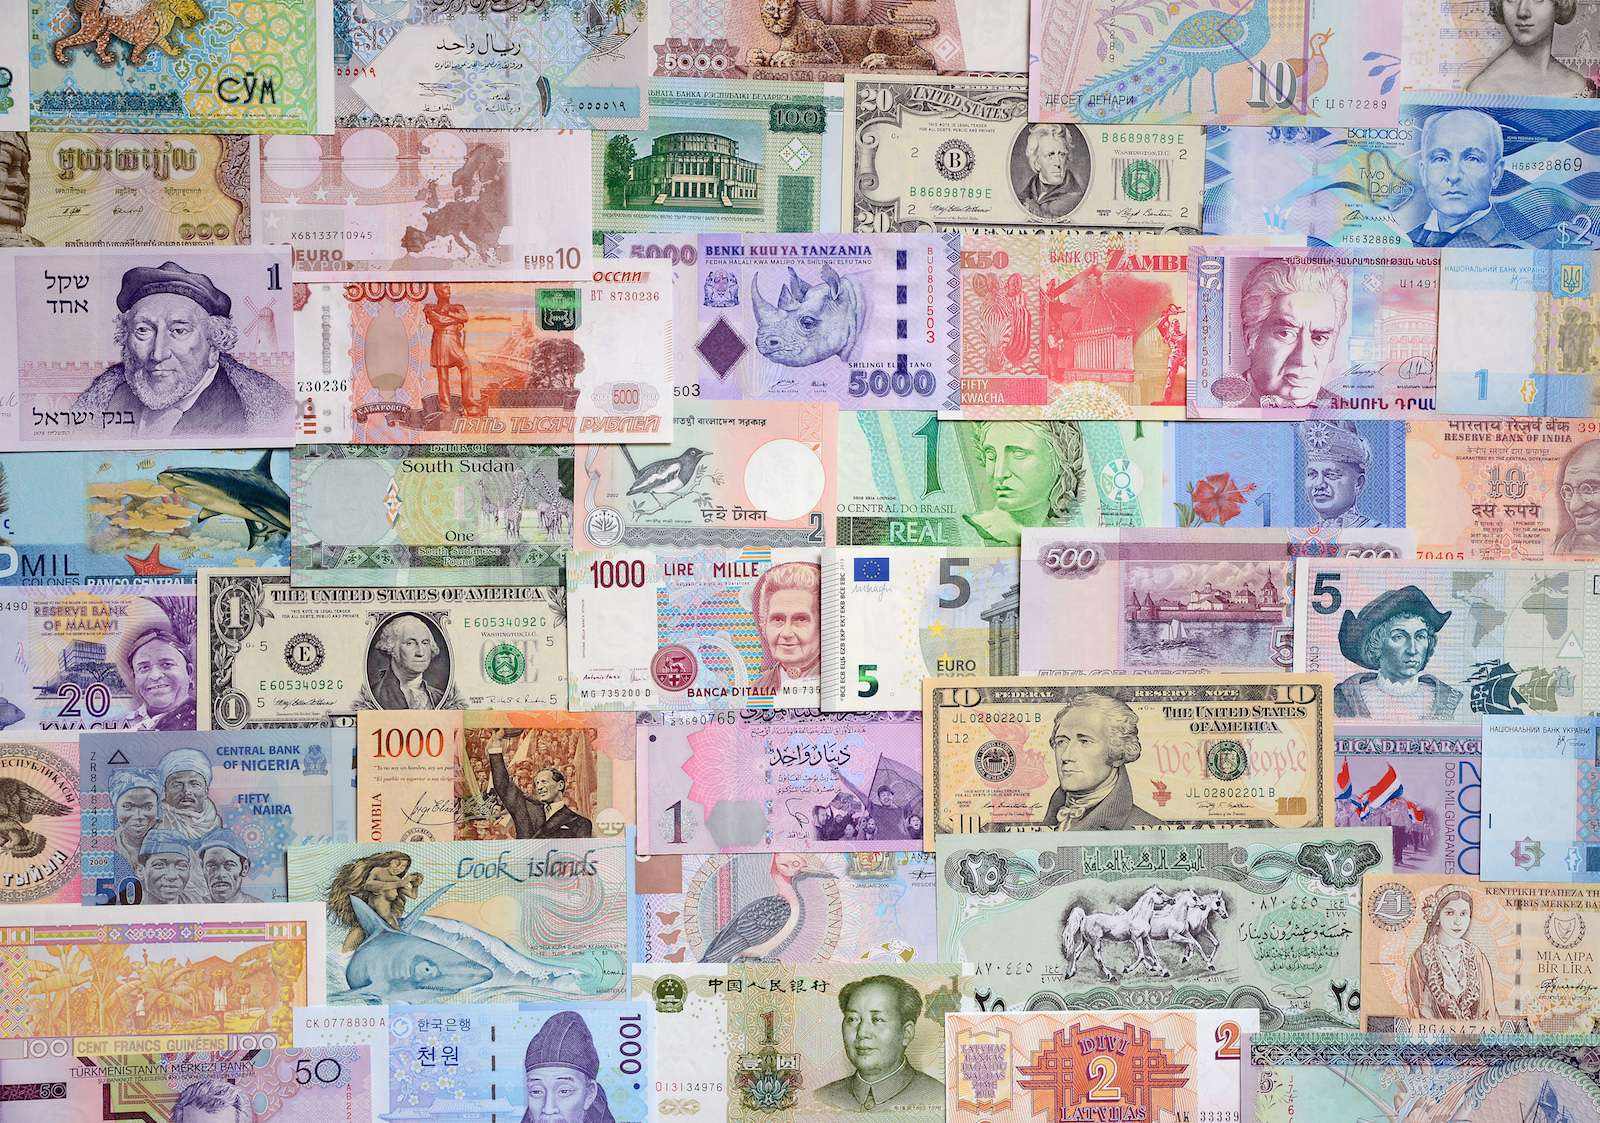
\includegraphics[width=0.6\linewidth]{Banknotes.jpg}\\ 
	\text{Fonte: \cite{BRIT}}
\end{figure}

 
\section{Uma nova era: Cartões e ATMs}

Com a evolução da tecnologia, dinheiro e pagamentos mudaram drasticamente a partir daqui. A tecnologia atual de processamento de cartões e as soluções de negócios avançadas tornam as transações financeiras possíveis de praticamente qualquer lugar de forma instantânea.  Tudo isto começou a ser possível a partir de 1871 quando a Western Union(WU) \footnote{Western Union é o nome pelo qual conhemos a companhia hoje, seu nome em específico era então Western Union Telegraph Company} deu lançamento as EFTs\footnote{Do inglês, Electronic Fund Transfers, EFTs, que também eram conhecidos como wiring transfers.}, as transferências de fundos eletrônicos como método de pagamento para a troca de fundos. As EFTs tornaram-se populares como formas rápidas e fáceis de enviar dinheiro sem exigir uma troca física de dinheiro entre as partes remetentes e destinatárias tornando-se então a principal área de negócios da WU.\\
Pouco menos de cem anos depois, já no findar do século XX, surgiu  um dos objetos mais importantes atualmente. Descrito como um pequeno cartão de plástico de precisamente 85,60 x 53,98 milímetros com cantos arredondados, que pode ser usado em praticamente qualquer lugar do mundo, ou online, para fazer pagamentos ou sacar dinheiro. Hoje chamamos este objeto de cartão de crédito ou débito. 
Mas não poderiamos deixar de citar que um pouco antes disto em 1967 na torre Enfield ao norte de Londres inaugurou-se então o primeiro caixa eletrônico (ATM)\footnote{Também segundo \cite{QUARTZ}}\footnote{A sigla ATM vem do inglês, que significa "Automated Teller Machine". Os Tellers eram funcionários dos bancos que ficavam responsáveis por realizar as transações diretamente com os clientes bancários. No Brasil, a expressão "na boca do caixa" representa bem essa interação com os tellers.}. Os ATMs são dispositivos de telecomunicações eletrônicas que permitem aos clientes de instituições financeiras realizar transações como saques em dinheiro, transferências, consultas de saldos e depósitos a qualquer momento do dia ou da noite e sem a necessidade de interação humana, ou seja, sem contato direto com funcionários de instituições financeiras.

\begin{citacao}
	Na época, os cartões bancários de plástico ainda não haviam sido inventados, então a máquina recebia cheques e distribuía apenas \pounds10 por vez. (Sendo justo, isto vale cerca de \pounds370 em dinheiro de hoje.) John Shepherd-Barron, que inventou o primeiro caixa eletrônico, morreu em 2010 um mês antes de seu 85º aniversário. Ele disse que a ideia foi inspirada em um dispensador de barra de chocolate. (Tradução Livre) \cite{QUARTZ}
\end{citacao}

Hoje em dia os ATMs são muito conhecidos e utilizados por serem  umas das formas principais de movimentação monetária física nos  bancos. São conhecidos por estar presentes nos maiores estabelecimentos e estações de grande fluxo de pessoas como aeroportos, rodoviárias e centros comerciais. 



\section{Transações eletrônicas: dinheiro e bancos digitais}
Ainda se tratando de tecnologia, devido a grande melhoria nas conectividades e nos hardwares dos dispositivos surgiu então uma nova forma de se tratar com dinheiro. Tal o conhecemos como o dinheiro digital, que refere-se a qualquer meio de pagamento gerenciado, armazenado ou transacionado de forma eletrônica por meio de sistemas computadorizados, especialmente pela Internet. 
Um marco na evolução dos pagamentos digitais ocorreu em 1998 com o lançamento do Paypal\footnote{De acordo com	 \cite{CTECH}, Fundada por Max Levchin, Peter Thiel, Luke Nosek e Ken Howery, a PayPal foi criada, inicialmente, como uma solução para pagamentos via Palm Pilot. Após a fusão com a X.com, o PayPal passou a atuar na internet, tornando-se uma das plataformas de pagamentos online mais populares do mundo. Atualmente oferece um sistema de pagamentos on-line que é uma alternativa eletrônica aos métodos de pagamento tradicionais, como cheques e ordens de pagamento.}, que permitia a transferência e armazenamento de valores eletrônicos em carteira eletônica, iniciando uma febre nesse ramo. No Brasil, a digitalização das operações financeiras deu início com o surgimento dos boletos bancário no fim dos anos 90 e da Transferência Eletrônica Disponível\footnote{O TED foi introduzido em 23 de abril de 2002 pela circular n° 3.115 do Banco Central do Brasil. Veja em \cite{BCB}} (TED), logo no início  dos anos 2000, mas seu grande fomento surgiu no começo dos anos 2010, quando surgiram os primeiros bancos digitais no Brasil, que chegaram com fortes diferenciais  para a época, como a gratuidade em diversos serviços como transferências entre contas, documentos de crédito(DOCs) e TEDs, alguns tipos de investimento, rendimento acima da Poupança na própria conta corrente, além de outros diferenciais como cartão de crédito sem anuidade e conta corrente totalmente gratuita.\footnote{Leia mais sobre a digitalização dos bancos em \cite{DOMINA}} As fintechs, como são conhecidas tais instituições financeiras, puderam gerar uma maior evolução das instituições tradicionais devido a concorrência fazendo ainda que tais empresas criassem suas próprias versões digitais.\ \\

No próximo capítulo falaremos sobre um subconjunto do dinheiro digital, o dinheiro virtual. 

\begin{figure}[H]
	\centering
	\caption{Resumo do capítulo em uma imagem}
	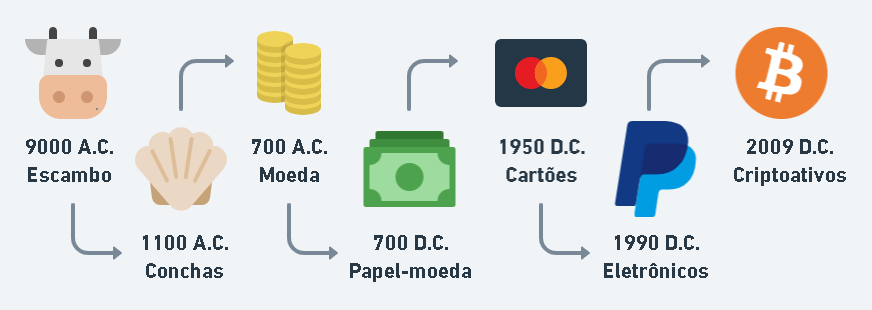
\includegraphics[width=\linewidth]{Resumo.png}
	\text{Fonte: Desenvolvido pelo autor com assets disponíveis em \cite{WHIM}}\\
\end{figure}




